% --------------------------------------------------------------
% This is all preamble stuff that you don't have to worry about.
% Head down to where it says "Start here"
% --------------------------------------------------------------
 
\documentclass[12pt]{article}
 
\usepackage{float} 
\usepackage[margin=1in]{geometry} 
\usepackage{amsmath,amsthm,amssymb}
\usepackage{listings}
\usepackage{enumitem}   
\usepackage{graphicx}
\graphicspath{ {./images/} }

\lstset{
   basicstyle=\fontsize{8}{9}\selectfont\ttfamily
}
 
\begin{document}
 
% --------------------------------------------------------------
%                         Start here
% --------------------------------------------------------------
 
%\renewcommand{\qedsymbol}{\filledbox}
 
\title{Homework 6}%replace X with the appropriate number
\author{Hai Nguyen \& Huan Nguyen\\ %replace with your name
STAT760 - Statistical Learning} %if necessary, replace with your course title
\maketitle
\textbf{Problem 1}
\\Find the mean of each of the ten classes and also the first 3 principal components for
each class. You will have to add some random noise to the covariance matrices to make
them have determinant different than zero. You can use built-in functions in your
programming language for finding eigenvectors and eigenvalues.
\\Show the mean of each class as a little picture 16x16 and also each of the tree principal
components as a 16x16 picture.\\
\textit{MATLAB code:}
\begin{lstlisting}
clear all
close all
A = load('zip.train');
N = size(A,1);
noise_level = 0.001;
mean = zeros(10,256);
cnt = zeros(10,1);
cov_mat = zeros(256,256,10);
I_mean = zeros(16,16,10);

for i=1:N
    mean(A(i,1)+1, :) = mean(A(i,1)+1, :) + A(i,2:end);    
    cnt(A(i,1)+1) = cnt(A(i,1)+1) + 1;
end

for i=1:10
    mean(i, :) = mean(i, :) / cnt(i);
    m = reshape(mean(i,:),[16 16]);
    I_mean(:,:,i) = mat2gray(m,[-1 1])';
end

for i=1:N
    tmp = A(i,2:end) - mean(A(i,1)+1,:);
    cov_mat(:,:,A(i,1)+1) = cov_mat(:,:,A(i,1)+1) + (tmp' * tmp); 
end

for i=1:10
    cov_mat(:,:,i) = cov_mat(:,:,i) / cnt(i) + noise_level * eye(256);
    
    [V,D] = eig(cov_mat(:,:,i));
    [d,ind] = sort(diag(D),'descend');
    Ds = D(ind,ind);
    Vs = V(:,ind);

    figure
    subplot(2,2,1)
    imshow(I_mean(:,:,i));
    title(strcat('Mean of digit ', num2str(i-1)));    

    m = reshape(Vs(:,1),[16 16]);
    I = mat2gray(m,[-1 1]);
    subplot(2,2,2)
    imshow(I');
    title('1st principal component'); 
    
    m = reshape(Vs(:,2),[16 16]);
    I = mat2gray(m,[-1 1]);
    subplot(2,2,3)
    imshow(I');
    title('2nd principal component'); 
    
    m = reshape(Vs(:,3),[16 16]);
    I = mat2gray(m,[-1 1]);
    subplot(2,2,4)
    imshow(I');
    title('3rd principal component');     
end
\end{lstlisting}
\textit{Results:}
\begin{figure}[H]
\begin{center}
    \caption{Digit 0}
    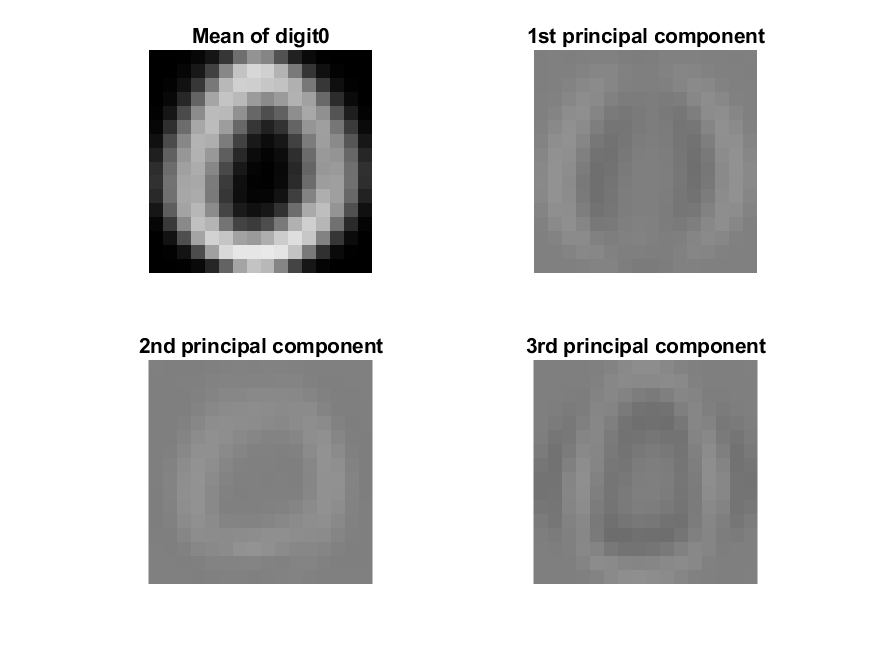
\includegraphics[width=0.75\textwidth]{images/digit0.png}
\end{center}
\end{figure}

\begin{figure}[H]
\begin{center}
    \caption{Digit 1}
    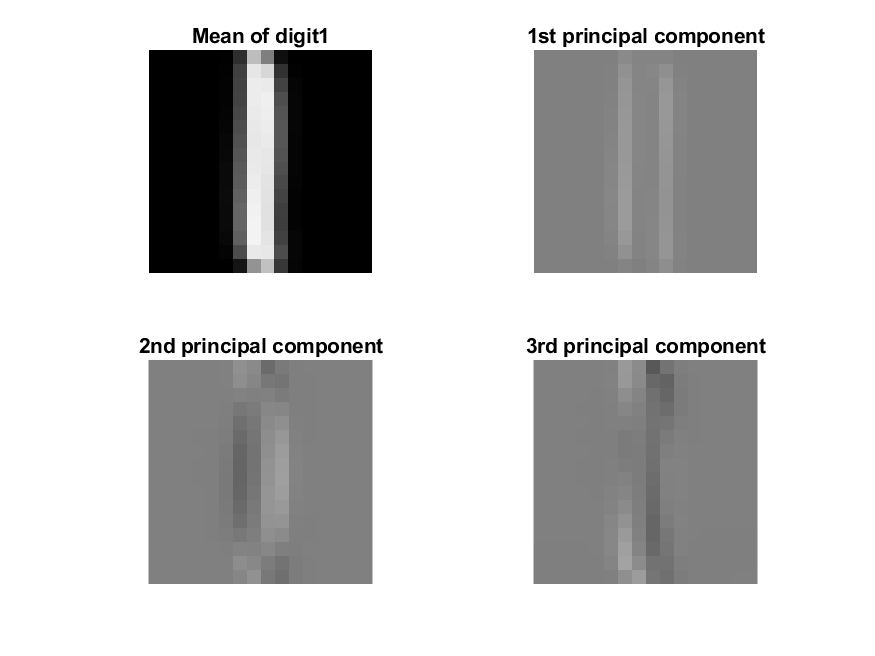
\includegraphics[width=0.75\textwidth]{images/digit1.png}
\end{center}
\end{figure}

\begin{figure}[H]
\begin{center}
    \caption{Digit 2}
    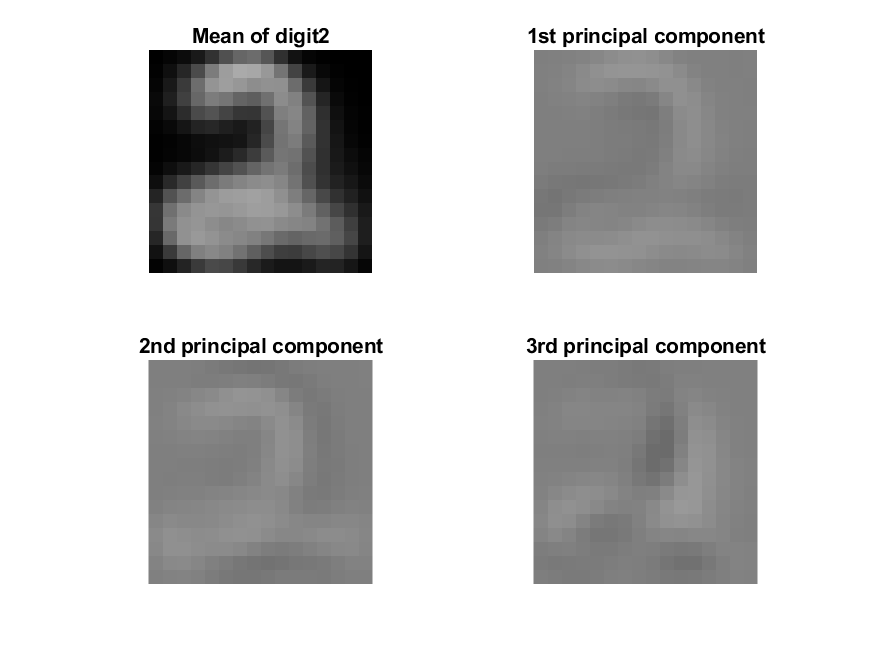
\includegraphics[width=0.75\textwidth]{images/digit2.png}
\end{center}
\end{figure}

\begin{figure}[H]
\begin{center}
    \caption{Digit 3}
    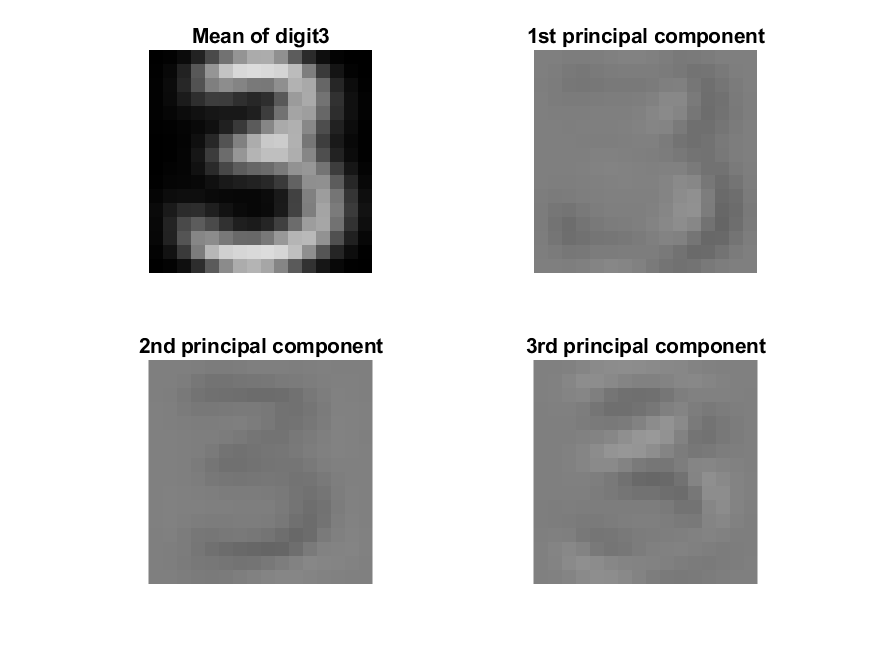
\includegraphics[width=0.75\textwidth]{images/digit3.png}
\end{center}
\end{figure}

\begin{figure}[H]
\begin{center}
    \caption{Digit 4}
    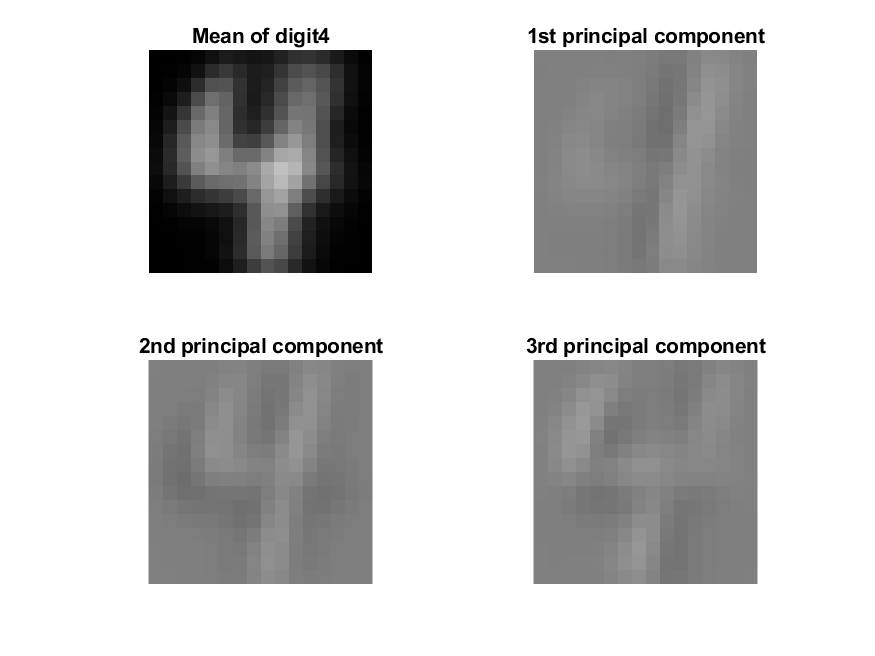
\includegraphics[width=0.75\textwidth]{images/digit4.png}
\end{center}
\end{figure}

\begin{figure}[H]
\begin{center}
    \caption{Digit 5}
    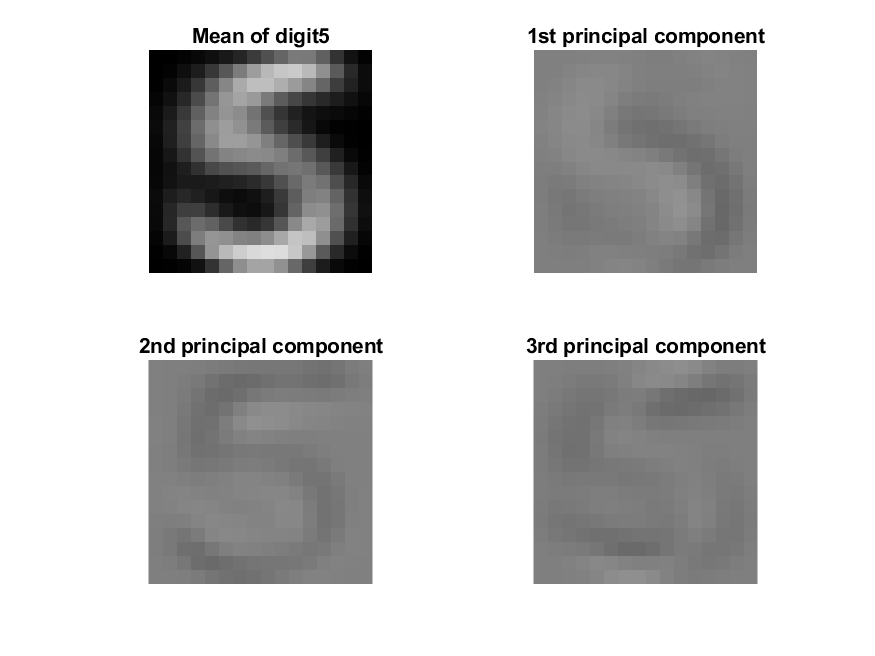
\includegraphics[width=0.75\textwidth]{images/digit5.png}
\end{center}
\end{figure}

\begin{figure}[H]
\begin{center}
    \caption{Digit 6}
    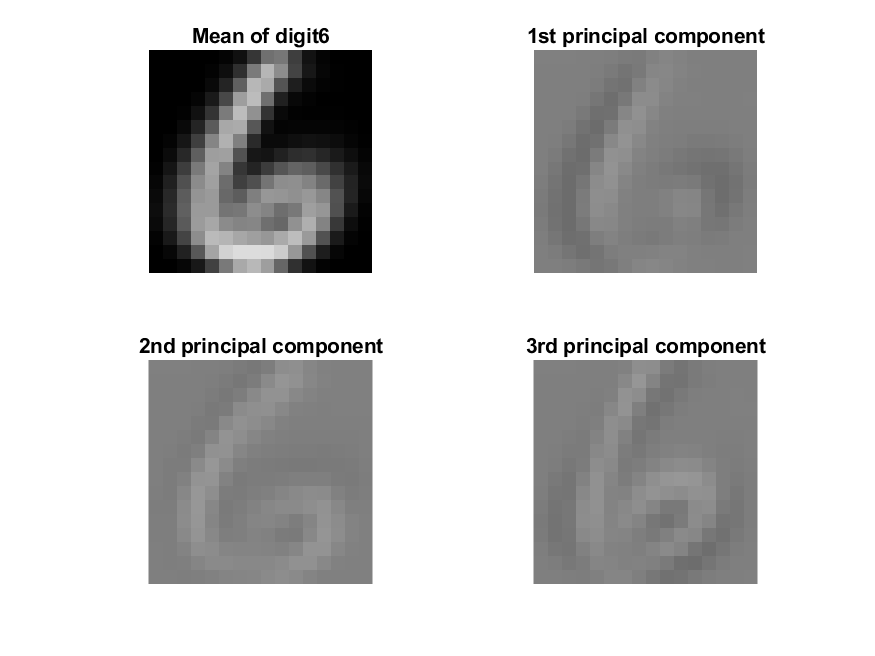
\includegraphics[width=0.75\textwidth]{images/digit6.png}
\end{center}
\end{figure}

\begin{figure}[H]
\begin{center}
    \caption{Digit 7}
    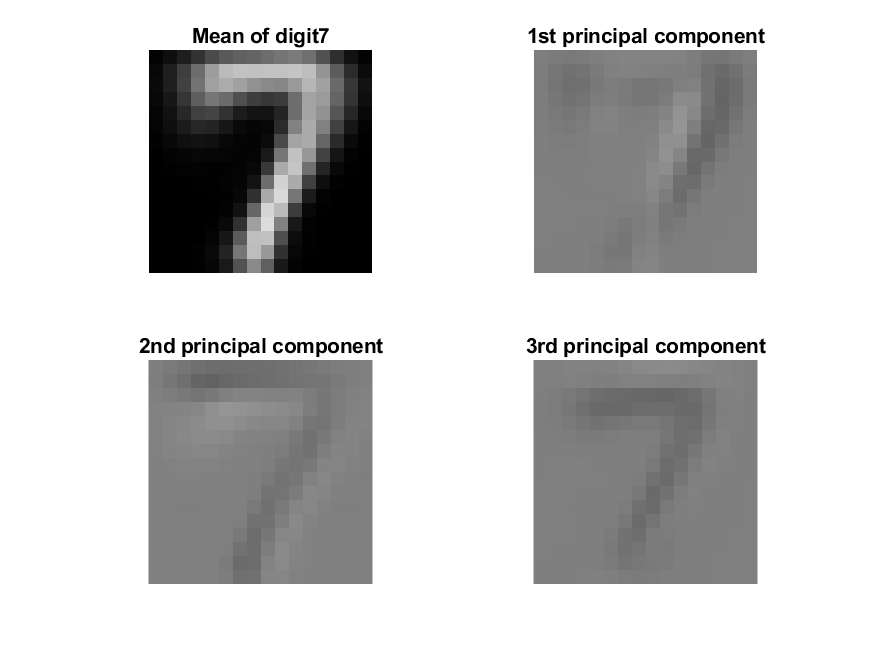
\includegraphics[width=0.75\textwidth]{images/digit7.png}
\end{center}
\end{figure}

\begin{figure}[H]
\begin{center}
    \caption{Digit 8}
    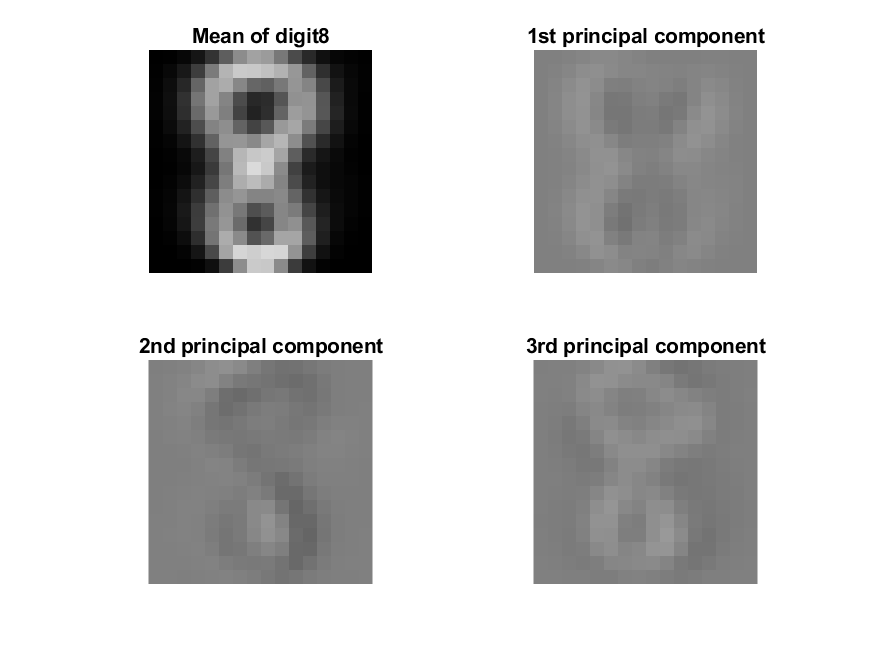
\includegraphics[width=0.75\textwidth]{images/digit8.png}
\end{center}
\end{figure}

\begin{figure}[H]
\begin{center}
    \caption{Digit 9}
    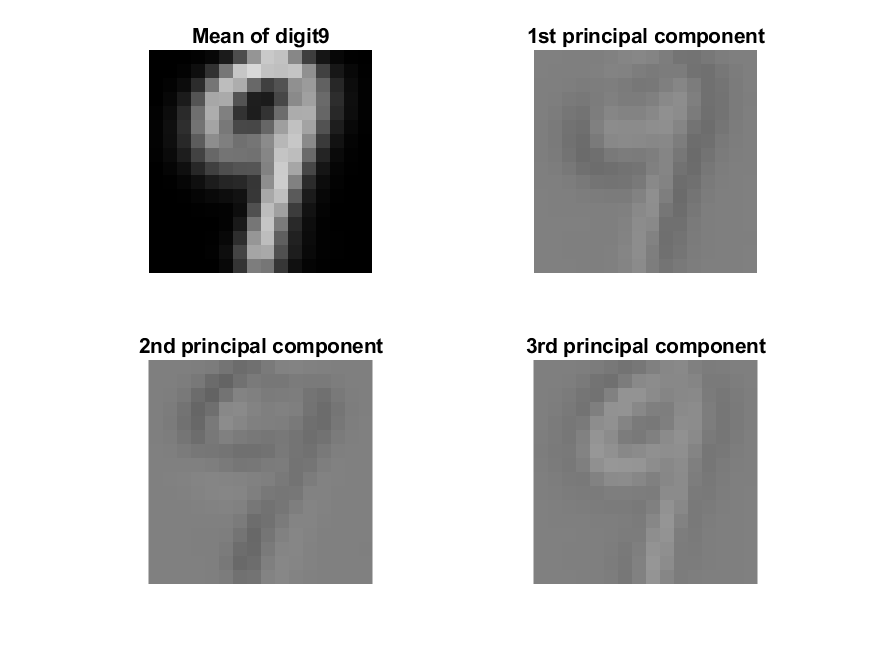
\includegraphics[width=0.75\textwidth]{images/digit9.png}
\end{center}
\end{figure}

\textbf{Problem 2}
\\This problem refers to Chapter 4 of Neural Networks, Springer-Verlag (Perceptron Learning).
\\Create a linearly separable training set with two classes P and N (in two dimensions, ten points
each class). Find the separating line using the perceptron learning algorithm. Stop the
algorithm when the classes have been separated. Plot the result.
\begin{itemize}
    \item Generate data: 
\begin{lstlisting}
close all
clear all
clc

% Number of samples of each class
Sample = 10;

% Define inputs and outputs
offset = 5; % offset for second class
x_org = [randn(2,Sample) randn(2,Sample)+offset]; 
y_org = [zeros(1,Sample) ones(1,Sample)]; 
\end{lstlisting}
\item Perceptron learning
\begin{lstlisting}
% Extended vector
x_ext = vertcat(x_org, ones(1,2*Sample));

% % Start: The weight vector w_0 is generated randomly,
w = rand(1,3);

% Test: Select randomly a vector x from P U N
while 1  
    % Check stop condition: stop when all vectors are classified correctly
    y_est_all = w * x_ext;
    y_est_all = y_est_all > 0;
    if isequal(y_est_all, logical(y_org))
        break;
    end
    
    random_int = randi(length(x_ext));
    x_rand = x_ext(:, random_int);

    y_est = w * x_rand;
    y_true = y_org(random_int);    

    if (y_true == 1) && (y_est <= 0)
        w = w + x_rand';
    end

    if (y_true == 0) && (y_est > 0)
        w = w - x_rand';
    end
        
end

plotpv(x_org,y_org);
plotpc(w(:,1:end-1),w(end));
grid on
\end{lstlisting}
\item Figures
\begin{figure}[H]
\begin{center}
  \caption{Perceptron learning.}
  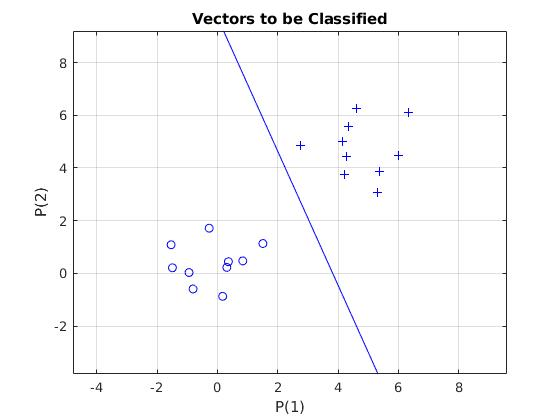
\includegraphics[width=0.75\textwidth]{images/Fig2-1.jpg}
 \end{center}
\end{figure}
\end{itemize}
Train the same set using gradient descent on the error function for a sigmoidal activation function. Plot the separating boundary for threshold 0.5.
\begin{itemize}
    \item Helper functions:
    
    \begin{itemize}
        \item plotData

    
    \begin{lstlisting}
function plotData(X, y)

% Create New Figure
figure; hold on;

% Find Indices of Positive and Negative Examples
pos = find(y==1); neg = find(y == 0);
% Plot Examples
plot(X(pos, 1), X(pos, 2), 'k+','LineWidth', 2, ...
'MarkerSize', 7);
plot(X(neg, 1), X(neg, 2), 'ko', 'MarkerFaceColor', 'y', ...
'MarkerSize', 7);

hold off;

end
    \end{lstlisting}
    
    \item plotDecisionBoundary
\begin{lstlisting}
function plotDecisionBoundary(theta, X, y)

% Plot Data
plotData(X(:,2:3), y);
hold on

% Only need 2 points to define a line, so choose two endpoints
plot_x = [min(X(:,2))-2,  max(X(:,2))+2];

% Calculate the decision boundary line
plot_y = (-1./theta(3)).*(theta(2).*plot_x + theta(1));

% Plot, and adjust axes for better viewing
plot(plot_x, plot_y)

end
hold off
grid on

end
\end{lstlisting}    

\item gradientDescent

\begin{lstlisting}
function [theta, J_history] = gradientDescent(X, y, theta, alpha, num_iters)

m = length(y); 
J_history = zeros(num_iters, 1);

for iter = 1:num_iters
  saved_theta = theta;  
  theta = theta - alpha*1/m*X'*(sigmoid(X*saved_theta)-y);  
  J_history(iter) = 1/m*sum(-y'*log(sigmoid(X*theta))-(1.-y)'*log(1-sigmoid(X*theta)));
end

end

\end{lstlisting}

        \end{itemize}

\item Main program:
\begin{lstlisting}
%% Logistic Regression
x = x_org';
y = y_org';
[m, n] = size(x); 

x = [ones(m, 1) x];

initial_theta = zeros(n + 1, 1);
iterations = 2500;
alpha = 0.025;

[theta, J] = gradientDescent(x, y, initial_theta, alpha, iterations);

% Plot Boundary
plotDecisionBoundary(theta, x, y);
grid on

\end{lstlisting}

\item Decision boundary:
\begin{figure}[H]
\begin{center}
  \caption{Decision boundary.}
  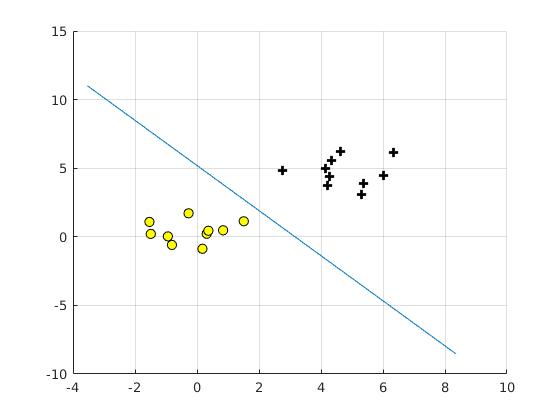
\includegraphics[width=0.75\textwidth]{images/Fig2-2.jpg}
 \end{center}
\end{figure}
\end{itemize}
% --------------------------------------------------------------
%     You don't have to mess with anything below this line.
% --------------------------------------------------------------
 
\end{document}